\documentclass{article}

% Required packages
\usepackage{amssymb}
\usepackage{amsmath}
\usepackage{graphicx}
\usepackage{geometry}
\usepackage{tikz}
\usepackage{array}
\usepackage{booktabs}
\usepackage{enumitem}
\usepackage{listings}
\usepackage{xcolor}
\usepackage{fancyhdr}
\usepackage{float}
\usepackage{subcaption}

% Set page geometry
\geometry{a4paper, margin=1in}

% Configure listings for Python
\lstset{
  language=Python,
  basicstyle=\ttfamily\footnotesize,
  numbers=left,
  numberstyle=\tiny\color{gray},
  frame=single,
  breaklines=true,
  breakatwhitespace=true,
  captionpos=b,
  tabsize=4,
  showspaces=false,
  showstringspaces=false,
  showtabs=false,
  commentstyle=\color{gray}\textit,
  keywordstyle=\color{blue}\bfseries,
  stringstyle=\color{red}
}

\begin{document}


\pagestyle{fancy}
\chead{DSC 255: Machine Learning Fundamentals (Spring 2025)}
\lhead{Homework 3}
\rhead{Randall Rogers}

\subsection*{Solution 1 (a)}

\noindent\rule{\textwidth}{0.4pt}\\

$$\boldsymbol{\mu} = [\mu_x, \mu_y]^T$$\\
$$\boldsymbol{\Sigma} = \begin{bmatrix} \sigma_x^2 & \rho\sigma_x\sigma_y \\ \rho\sigma_x\sigma_y & \sigma_y^2 \end{bmatrix}$$

\begin{itemize}
    \item Mean vector: $\boldsymbol{\mu}$
    \item Covariance matrix: $\boldsymbol{\Sigma}$
\end{itemize}

\parbox{\textwidth}{Let $\mu_x = 2$, $\mu_y = 2$, $\sigma_x = 1$, $\sigma_y = 0.5$, and $\rho = -0.5$}\\

\parbox{\textwidth}{Solve for mean vector $\boldsymbol{\mu}$:}\\

$$\boldsymbol{\mu} = \begin{bmatrix} \mu_x & \mu_y \end{bmatrix}^T = \begin{bmatrix}
    \mu_x \\
    \mu_y
\end{bmatrix} = \begin{bmatrix}
    2 \\
    2
\end{bmatrix}$$\\

\parbox{\textwidth}{Solve for covariance matrix $\boldsymbol{\Sigma}$:}\\

$$\boldsymbol{\Sigma} = \begin{bmatrix} \sigma_x^2 & \rho\sigma_x\sigma_y \\ \rho\sigma_x\sigma_y & \sigma_y^2 \end{bmatrix} = \begin{bmatrix} 1^2 & (-0.5)(1)(0.5) \\(-0.5)(1)(0.5) & 0.5^2\end{bmatrix} = \begin{bmatrix} 1 & -0.25 \\-0.25 & 0.25\end{bmatrix}$$\\

\parbox{\textwidth}{$\therefore$ the bivariate Gaussian has parameters:}\\

$$\mathcal{N}(\boldsymbol{\mu},\boldsymbol{\Sigma})=\mathcal{N}\left(\begin{bmatrix} 2 \\ 2 \end{bmatrix}, \begin{bmatrix} 
    1 & -0.25 \\
    -0.25 & 0.25
\end{bmatrix}\right)$$

\noindent\rule{\textwidth}{0.4pt}\\

\newpage

\subsection*{Solution 1 (b)}

\noindent\rule{\textwidth}{0.4pt}\\

\parbox{\textwidth}{For a bivariate Gaussian distribution, we need to specify the following parameters:}\\

$$\boldsymbol{\mu} = [\mu_x, \mu_y]^T$$\\
$$\boldsymbol{\Sigma} = \begin{bmatrix} \sigma_x^2 & \rho\sigma_x\sigma_y \\ \rho\sigma_x\sigma_y & \sigma_y^2 \end{bmatrix}$$

\begin{itemize}
    \item Mean vector: $\boldsymbol{\mu}$
    \item Covariance matrix: $\boldsymbol{\Sigma}$
\end{itemize}

\parbox{\textwidth}{Let $\mu_x = 1$, $\mu_y = 2$, $\sigma_x = 1$, $\sigma_y = 0$}\\

\parbox{\textwidth}{Solve for mean vector $\boldsymbol{\mu}$:}\\

$$\boldsymbol{\mu} = \begin{bmatrix} \mu_x & \mu_y \end{bmatrix}^T = \begin{bmatrix}
    \mu_x \\
    \mu_y
\end{bmatrix} = \begin{bmatrix}
    1 \\
    2
\end{bmatrix}$$\\

\parbox{\textwidth}{Solve for covariance matrix $\boldsymbol{\Sigma}$:}\\

$$\boldsymbol{\Sigma} = \begin{bmatrix} \sigma_x^2 & \rho\sigma_x\sigma_y \\ \rho\sigma_x\sigma_y & \sigma_y^2 \end{bmatrix} = \begin{bmatrix} 1^2 & 0 \\ 0 & 0^2\end{bmatrix} = \begin{bmatrix} 1 & 0 \\ 0 & 0\end{bmatrix}$$\\

\parbox{\textwidth}{$\therefore$ the bivariate Gaussian has parameters:}\\

$$\mathcal{N}(\boldsymbol{\mu},\boldsymbol{\Sigma})=\mathcal{N}\left(\begin{bmatrix} 1 \\ 2 \end{bmatrix}, \begin{bmatrix} 
    1 & 0 \\
    0 & 0
\end{bmatrix}\right)$$

\noindent\rule{\textwidth}{0.4pt}\\

\newpage

\subsection*{\parbox{\textwidth}{\textbf{Solution 2}}}
\noindent\rule{\textwidth}{0.4pt}\\

\subsubsection*{Step 1}

\parbox{\textwidth}{The Bayesian decision rule for generative classifiers is defined as:}

\vspace{0.2cm}

$$\hat{y} = \arg\max_{y \in \{+,-\}} p(y|x) = \arg\max_{y \in \{+,-\}} \frac{p(x|y)p(y)}{p(x)}$$

\begin{itemize}
\item \parbox{\textwidth}{Since $p(x)$ is constant for both classes, the decision rule simplifies to:}
\end{itemize}

$$\hat{y} = \arg\max_{y \in \{+,-\}} p(x|y)p(y)$$

\subsubsection*{Step 2}

\parbox{\textwidth}{The $(+)$ class is predicticted when the folowing holds:}

\vspace{0.2cm}

$$p(x|+)p(+) > p(x|-)p(-)$$

\subsubsection*{Step 3} 

\parbox{\textwidth}{Identify possible reasons for always predicting the positive class.}

\vspace{0.2cm}

\begin{enumerate}
    \item \textbf{Highly imbalanced prior probabilities:} If $p(+) \gg p(-)$, the classifier might always predict the positive class because the prior term dominates the decision, regardless of the likelihood term. This occurs when the training data contains many more $+$ examples than $-$ ones.
    
    \item \textbf{Poor estimation of class-conditional densities:} If $p(x|+)$ is consistently overestimated or $p(x|-)$ is consistently underestimated across the input space, the classifier will favor the $+$ class.
\end{enumerate}

\parbox{\textwidth}{$\therefore$ the classifier that predicts $+$ for all points $x$ in the input space is likely due to a combination of highly imbalanced prior probabilities and poor estimation of class-conditional densities.}
\noindent\rule{\textwidth}{0.4pt}\\

\newpage

\subsection*{Solution 3 (a)}

\noindent\rule{\textwidth}{0.4pt}\\

\subsubsection*{Step 1}
\parbox{\textwidth}{From Bayes Theorem we have:}
$$p(y|x) = \frac{p(x|y)p(y)}{p(x)}$$
$$or$$
$$p(y|x) \propto p(x|y)p(y)$$

\subsubsection*{Step 2}
\parbox{\textwidth}{The class probabilities are given as: }\\
$$\pi_1 = 0.33 \hspace{0.2cm} \pi_2 = 0.39 \hspace{0.2cm} \pi_3 = 0.28$$
\parbox{\textwidth}{From the plot the density for each class is:}
$$P(x=12.0|Class_1) = 0.4 \hspace{0.2cm} P(x=12.0|Class_2) = 0.05 \hspace{0.2cm} P(x=12.0|Class_3) = 0.0025$$

\subsubsection*{Step 3}

\parbox{\textwidth}{Use class probabilities and densities from \textit{Step 2}, the apply Bayes Theorem}\\

$P(Class_1|x=12.0) \propto P(x=12.0|Class_1)P(Class_1) = 0.4 \times 0.33 = 0.132$\\

$P(Class_2|x=12.0) \propto P(x=12.0|Class_2)P(Class_2) = 0.05 \times 0.39 = 0.0195$\\

$P(Class_3|x=12.0) \propto P(x=12.0|Class_3)P(Class_3) = 0.0025 \times 0.28 = 0.0007$\\

\parbox{\textwidth}{$\therefore$ the label $Class_1$ would be assigned at x=12.0}\\

\noindent\rule{\textwidth}{0.4pt}\\

\newpage

\subsection*{Solution 3 (b)}

\noindent\rule{\textwidth}{0.4pt}\\

\subsubsection*{Step 1}
\parbox{\textwidth}{From Bayes Theorem we have:}
$$p(y|x) = \frac{p(x|y)p(y)}{p(x)}$$
$$or$$
$$p(y|x) \propto p(x|y)p(y)$$

\subsubsection*{Step 2}
\parbox{\textwidth}{The class probabilities are given as: }\\
$$\pi_1 = 0.33 \hspace{0.2cm} \pi_2 = 0.39 \hspace{0.2cm} \pi_3 = 0.28$$
\parbox{\textwidth}{From \textit{Figure 1}, the density for each class is:}
$$P(x=12.5|Class_1) = 0.6 \hspace{0.2cm} P(x=12.5|Class_2) = 0.3 \hspace{0.2cm} P(x=12.5|Class_3) = 0.05$$

\subsubsection*{Step 3}

\parbox{\textwidth}{Use class probabilities and densities from \textit{Step 2}, then apply Bayes Theorem}\\

$P(Class_1|x=12.5) \propto P(x=12.5|Class_1)P(Class_1) = 0.6 \times 0.33 = 0.198$\\

$P(Class_2|x=12.5) \propto P(x=12.5|Class_2)P(Class_2) = 0.3 \times 0.39 = 0.117$\\

$P(Class_3|x=12.5) \propto P(x=12.5|Class_3)P(Class_3) = 0.05 \times 0.28 = 0.014$\\

\parbox{\textwidth}{$\therefore$ the label $Class_1$ would be assigned at x=12.5}\\

\noindent\rule{\textwidth}{0.4pt}\\

\newpage
\subsection*{Solution 3 (c)}

\noindent\rule{\textwidth}{0.4pt}\\

\subsubsection*{Step 1}
\parbox{\textwidth}{From Bayes Theorem we have:}
$$p(y|x) = \frac{p(x|y)p(y)}{p(x)}$$
$$or$$
$$p(y|x) \propto p(x|y)p(y)$$

\subsubsection*{Step 2}
\parbox{\textwidth}{The class probabilities are given as: }\\
$$\pi_1 = 0.33 \hspace{0.2cm} \pi_2 = 0.39 \hspace{0.2cm} \pi_3 = 0.28$$
\parbox{\textwidth}{From \textit{Figure 1}, the density for each class is:}
$$P(x=13.0|Class_1) = 0.3 \hspace{0.2cm} P(x=13.0|Class_2) = 0.6 \hspace{0.2cm} P(x=13.0|Class_3) = 0.2$$

\subsubsection*{Step 3}

\parbox{\textwidth}{Use class probabilities and densities from \textit{Step 2}, then apply Bayes Theorem}\\

$P(Class_1|x=13.0) \propto P(x=13.0|Class_1)P(Class_1) = 0.3 \times 0.33 = 0.099$\\

$P(Class_2|x=13.0) \propto P(x=13.0|Class_2)P(Class_2) = 0.6 \times 0.39 = 0.234$\\

$P(Class_3|x=13.0) \propto P(x=13.0|Class_3)P(Class_3) = 0.2 \times 0.28 = 0.056$\\

\parbox{\textwidth}{$\therefore$ the label $Class_2$ would be assigned at x=13.0}\\

\noindent\rule{\textwidth}{0.4pt}\\
\newpage
\subsection*{Solution 3 (d)}

\noindent\rule{\textwidth}{0.4pt}\\

\subsubsection*{Step 1}
\parbox{\textwidth}{From Bayes Theorem we have:}
$$p(y|x) = \frac{p(x|y)p(y)}{p(x)}$$
$$or$$
$$p(y|x) \propto p(x|y)p(y)$$

\subsubsection*{Step 2}
\parbox{\textwidth}{The class probabilities are given as: }\\
$$\pi_1 = 0.33 \hspace{0.2cm} \pi_2 = 0.39 \hspace{0.2cm} \pi_3 = 0.28$$
\parbox{\textwidth}{From \textit{Figure 1}, the density for each class is:}
$$P(x=13.5|Class_1) = 0.1 \hspace{0.2cm} P(x=13.5|Class_2) = 0.7 \hspace{0.2cm} P(x=13.5|Class_3) = 0.4$$

\subsubsection*{Step 3}

\parbox{\textwidth}{Use class probabilities and densities from \textit{Step 2}, then apply Bayes Theorem}\\

$P(Class_1|x=13.5) \propto P(x=13.5|Class_1)P(Class_1) = 0.1 \times 0.33 = 0.033$\\

$P(Class_2|x=13.5) \propto P(x=13.5|Class_2)P(Class_2) = 0.7 \times 0.39 = 0.273$\\

$P(Class_3|x=13.5) \propto P(x=13.5|Class_3)P(Class_3) = 0.4 \times 0.28 = 0.112$\\

\parbox{\textwidth}{$\therefore$ the label $Class_2$ would be assigned at x=13.5}\\

\noindent\rule{\textwidth}{0.4pt}\\
\newpage
\subsection*{Solution 3 (e)}

\noindent\rule{\textwidth}{0.4pt}\\

\subsubsection*{Step 1}
\parbox{\textwidth}{From Bayes Theorem we have:}
$$p(y|x) = \frac{p(x|y)p(y)}{p(x)}$$
$$or$$
$$p(y|x) \propto p(x|y)p(y)$$

\subsubsection*{Step 2}
\parbox{\textwidth}{The class probabilities are given as: }\\
$$\pi_1 = 0.33 \hspace{0.2cm} \pi_2 = 0.39 \hspace{0.2cm} \pi_3 = 0.28$$
\parbox{\textwidth}{From \textit{Figure 1}, the density for each class is:}
$$P(x=14.0|Class_1) = 0.05 \hspace{0.2cm} P(x=14.0|Class_2) = 0.2 \hspace{0.2cm} P(x=14.0|Class_3) = 0.8$$

\subsubsection*{Step 3}

\parbox{\textwidth}{Use class probabilities and densities from \textit{Step 2}, then apply Bayes Theorem}\\

$P(Class_1|x=14.0) \propto P(x=14.0|Class_1)P(Class_1) = 0.05 \times 0.33 = 0.0165$\\

$P(Class_2|x=14.0) \propto P(x=14.0|Class_2)P(Class_2) = 0.2 \times 0.39 = 0.078$\\

$P(Class_3|x=14.0) \propto P(x=14.0|Class_3)P(Class_3) = 0.8 \times 0.28 = 0.224$\\

\parbox{\textwidth}{$\therefore$ the label $Class_3$ would be assigned at x=14.0}\\

\noindent\rule{\textwidth}{0.4pt}\\

\newpage

\subsection*{Solution 4 (a)}
\noindent\rule{\textwidth}{0.4pt}\\
\subsubsection*{Step 1}
\parbox{\textwidth}{Analyze $\mu$}\\
\begin{itemize}
    \item \parbox{\textwidth}{Since $\mu = \begin{bmatrix} 0 \\ 0 \end{bmatrix}$, the center of the Gaussian is at the origin.}\\
\end{itemize}
\subsubsection*{Step 2}
\parbox{\textwidth}{Analyze $\Sigma$}\\
\begin{itemize}
    \item \parbox{\textwidth}{The covariance matrix $\Sigma = \begin{bmatrix} 9 & 0 \\ 0 & 1 \end{bmatrix}$ indicates that the variance in the x-direction is 9 and in the y-direction is 1. This means that the Gaussian will be elongated along the x-axis.}\\
\end{itemize}
\subsubsection*{Step 3}
\parbox{\textwidth}{Look at the standard deviation to determine the shape, since $\Sigma$ is a diagonal matrix}\\ 

\begin{itemize}
    \item The standard deviation in the x-direction is $\sigma_x = \sqrt{9} = 3$
    \item The standard deviation in the y-direction is $\sigma_y = \sqrt{1} = 1$
\end{itemize}
\subsubsection*{Step 4}
\parbox{\textwidth}{Sketch the Gaussian}\\

\begin{center}
    \begin{tikzpicture}
        \draw[->] (-4,0) -- (4,0) node[right] {$x$};
        \draw[->] (0,-2) -- (0,2) node[above] {$y$};
        \draw[thick, blue] (0,0) ellipse (3 and 1);
        \node at (0,0) [circle, fill, inner sep=1pt]{};
        \node at (0.3,0.3) {$\mu$};
        \node at (3.0,0) [circle, fill, inner sep=1pt]{};
        \node at (3.5,0.3) {$\sigma_x = 3$};
        \node at (0,1.0) [circle, fill, inner sep=1pt]{};
        \node at (0.7,1.3) {$\sigma_y = 1$};
    \end{tikzpicture}
\end{center}

\noindent\rule{\textwidth}{0.4pt}\\

\newpage

\subsection*{Solution 4 (b)}

\noindent\rule{\textwidth}{0.4pt}\\

\subsubsection*{Step 1}
\parbox{\textwidth}{Analyze $\mu$}\\
\begin{itemize}
    \item \parbox{\textwidth}{Since $\mu = \begin{bmatrix} 0 \\ 0 \end{bmatrix}$, the center of the Gaussian is at the origin.}\\
\end{itemize}

\subsubsection*{Step 2}
\parbox{\textwidth}{Analyze $\Sigma$}\\
\begin{itemize}
    \item \parbox{\textwidth}{The covariance matrix $\Sigma = \begin{bmatrix} 1 & -0.75 \\ -0.75 & 1 \end{bmatrix}$ has non-zero off-diagonal elements.}\\
    \item \parbox{\textwidth}{This indicates a correlation between variables.}\\
    \item \parbox{\textwidth}{The negative correlation ($-0.75$) means that as one variable increases, the other tends to decrease.}\\
    \item \parbox{\textwidth}{Look at the eigenvalues and eigenvectors to determine the shape since we don't have a diagonal matrix in this case.}\\
\end{itemize}

\subsubsection*{Step 3}
\parbox{\textwidth}{Find eigenvalues and eigenvectors}\\ 
\begin{itemize}
    \item \parbox{\textwidth}{The eigenvalues of $\Sigma$ are $\lambda_1 = 1 + 0.75 = 1.75$ and $\lambda_2 = 1 - 0.75 = 0.25$.}\\
    \item \parbox{\textwidth}{The corresponding eigenvectors are $v_1 = \begin{bmatrix} 1 \\ -1 \end{bmatrix}$ and $v_2 = \begin{bmatrix} 1 \\ 1 \end{bmatrix}$.}\\
    \item \parbox{\textwidth}{The standard deviations along the principal axes are $\sigma_1 = \sqrt{1.75} \approx 1.32$ and $\sigma_2 = \sqrt{0.25} = 0.5$.}\\
\end{itemize}

\subsubsection*{Step 4}
\parbox{\textwidth}{Sketch the Gaussian}\\
\begin{center}
    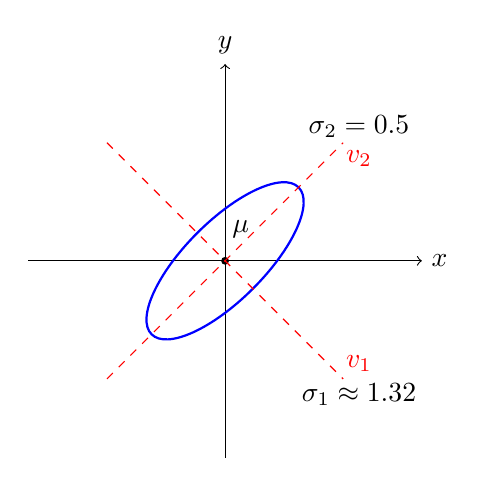
\begin{tikzpicture}
        \draw[->] (-2.5,0) -- (2.5,0) node[right] {$x$};
        \draw[->] (0,-2.5) -- (0,2.5) node[above] {$y$};
        \draw[thick, blue, rotate=45] (0,0) ellipse (1.32 and 0.5);
        \node at (0,0) [circle, fill, inner sep=1pt]{};
        \node at (0.2,0.4) {$\mu$};
        \draw[dashed, red] (-1.5,-1.5) -- (1.5,1.5) node at (1.7,1.3) {$v_2$};
        \draw[dashed, red] (-1.5,1.5) -- (1.5,-1.5) node at (1.7,-1.3) {$v_1$};
        \node at (1.7,-1.7) {$\sigma_1 \approx 1.32$};
        \node at (1.7,1.7) {$\sigma_2 = 0.5$};
    \end{tikzpicture}
\end{center}

\noindent\rule{\textwidth}{0.4pt}\\

\newpage
\subsection*{Solution 5}
\noindent\rule{\textwidth}{0.4pt}\\
\parbox{\textwidth}{A unit vector in $\mathbb{R}^2$ is a vector of the form:}\\
$$\begin{bmatrix} x \\ y \end{bmatrix}$$
\parbox{\textwidth}{To be orthogonal to $\begin{bmatrix} 1 \\ 1 \end{bmatrix}$, the dot product must equal zero:}\\
$$\begin{bmatrix} 1 \\ 1 \end{bmatrix} \cdot \begin{bmatrix} x \\ y \end{bmatrix} = 0$$
\parbox{\textwidth}{This gives the equation:}\\
$$x + y = 0$$
\parbox{\textwidth}{This means that $y = -x$.}\\
\parbox{\textwidth}{Now, we need to find the unit vectors. A unit vector has a magnitude of 1:}\\
$$\sqrt{x^2 + y^2} = 1$$
\parbox{\textwidth}{Substituting $y = -x$ into the equation:}\\
$$\sqrt{x^2 + (-x)^2} = 1$$
$$\sqrt{2x^2} = 1$$
$$\sqrt{2}|x| = 1$$
$$|x| = \frac{1}{\sqrt{2}}$$
\parbox{\textwidth}{This gives two solutions for $x$:}\\
$$x = \frac{1}{\sqrt{2}} \quad \text{or} \quad x = -\frac{1}{\sqrt{2}}$$
\parbox{\textwidth}{Substituting back to find $y$:}\\
$$y = -\frac{1}{\sqrt{2}} \quad \text{or} \quad y = \frac{1}{\sqrt{2}}$$
\parbox{\textwidth}{$\therefore$ the unit vectors orthogonal to $\begin{bmatrix} 1 \\ 1 \end{bmatrix}$ are:}\\
$$\begin{bmatrix} \frac{1}{\sqrt{2}} \\ -\frac{1}{\sqrt{2}} \end{bmatrix} \quad \text{and} \quad \begin{bmatrix} -\frac{1}{\sqrt{2}} \\ \frac{1}{\sqrt{2}} \end{bmatrix}$$

\noindent\rule{\textwidth}{0.4pt}\\

\newpage

\subsection*{Solution 6}
\noindent\rule{\textwidth}{0.4pt}\\
\parbox{\textwidth}{Let $x\cdot x = 25 ,\hspace{0.2cm} \forall \hspace{0.1cm} x \in \mathbb{R}^{d}$}\\
$$ x\cdot x = \|x\|^2 =25 \rightarrow \sqrt{\|x\|^2} = \sqrt{25} \rightarrow \|x\| = 5$$

\parbox{\textwidth}{Hence, the vector $x$ has a magnitude of 5.}\\

\parbox{\textwidth}{$\therefore$ the set of all points $x$ $\in$ $\mathbb{R}^d$ with $x \cdot x = 25$ is a sphere of radius 5 centered at the origin in $d$-dimensional space.}\\

\noindent\rule{\textwidth}{0.4pt}\\
\newpage
\subsection*{Solution 7}
\noindent\rule{\textwidth}{0.4pt}\\

\parbox{\textwidth}{The function $f(x) = 2x_1 - x_2 + 6x_3$ can be expressed in the form of a dot product:}\\

$$f(x) = w \cdot x$$\\

\parbox{\textwidth}{Where $w$ is a vector in $\mathbb{R}^3$ and $x$ is a vector in $\mathbb{R}^3$.}\\

\parbox{\textwidth}{We can then express $f(x)$ as the dot product of two matrices:}\\

$$f(x) = \begin{bmatrix} w_1 \\ w_2 \\ w_3 \end{bmatrix} \cdot \begin{bmatrix} x_1 \\ x_2 \\ x_3 \end{bmatrix} = w_1\cdot x_1 +w_2\cdot x_2 +w_3\cdot x_3$$

\parbox{\textwidth}{It follows that: $w_1 = 2 \hspace{0.2cm} w_2=-1 \hspace{0.2cm} w_3 = 6$}\\

\parbox{\textwidth}{$\therefore$ the vector $w$ is:}\\

$$w = \begin{bmatrix} 2 \\ -1 \\ 6 \end{bmatrix}$$

\noindent\rule{\textwidth}{0.4pt}\\
\newpage
\subsection*{Solution 8}
\noindent\rule{\textwidth}{0.4pt}\\

\parbox{\textwidth}{Let the dimensions of $A$ be $m \times n$ and the dimensions of $B$ be $n \times p$.}\\

\parbox{\textwidth}{The product $AB$ will have dimensions $m \times p$.}\\

\parbox{\textwidth}{Given that $AB$ has dimensions $10 \times 20$, and $A = m \times 30$.}\\

$$m = 10 \quad \hspace{0.3cm} \quad p = 20 \hspace{0.3cm} \quad n = 30$$\\

\parbox{\textwidth}{We know that the product $AB$ can be expressed as:}\\

$$AB = (m\times n)\boldsymbol{\times} (n\times p)$$

\parbox{\textwidth}{$\therefore$ the dimensions of $A$ and $B$ are:}\\
$$A: 10 \times 30$$
$$B: 30 \times 20$$

\noindent\rule{\textwidth}{0.4pt}\\

\newpage
\subsection*{Solution 9 (a)}
\noindent\rule{\textwidth}{0.4pt}\\

\parbox{\textwidth}{The matrix $X$ has $n$ rows and $d$ columns, so the dimension of $X$ is:}\\

$$X \in \mathbb{R}^{n \times d}$$

\parbox{\textwidth}{This means that $X$ has $n$ data points, each with $d$ features.}\\

\parbox{\textwidth}{$\therefore$ the dimension of $X$ is $n \times d$.}\\

\noindent\rule{\textwidth}{0.4pt}\\

\newpage
\subsection*{Solution 9 (b)}
\noindent\rule{\textwidth}{0.4pt}\\

\parbox{\textwidth}{The matrix ${XX}^T$ is the product of an $n \times d$ matrix and a $d \times n$ matrix.}\\

\parbox{\textwidth}{The resulting matrix will have dimensions $n \times n$.}\\

\parbox{\textwidth}{$\therefore$ the dimension of ${XX}^T$ is $n \times n$.}\\

\noindent\rule{\textwidth}{0.4pt}\\

\newpage
\subsection*{Solution 9 (c)}
\noindent\rule{\textwidth}{0.4pt}\\

\parbox{\textwidth}{The $(i,j)$ entry of ${X}^TX$ is the dot product of the $i$-th row of $X$ and the $j$-th column of $X^T$ }\\

\parbox{\textwidth}{This is simply the sum of the products of the corresponding elements:}\\

$$(X^TX)_{ij} = \sum_{k=1}^{d} x^{(i)}_k x^{(j)}_k$$

\parbox{\textwidth}{This is the inner product of the $i$-th and $j$-th data points.}\\

\parbox{\textwidth}{$\therefore$ the $(i,j)$ entry of ${X}^TX$ is the inner product of the $i$-th and $j$-th data points or $(x^{(n)},x^{(n)})$.}\\

\noindent\rule{\textwidth}{0.4pt}\\

\newpage
\subsection*{Solution 10}
\noindent\rule{\textwidth}{0.4pt}\\

\subsubsection*{Step 1}
\parbox{\textwidth}{Compute $x^{T}$}\\
$$x= \begin{bmatrix} 1 \\ 3 \\ 5 \end{bmatrix} \rightarrow x^{T} = \begin{bmatrix} 1 & 3 & 5 \end{bmatrix}$$

\subsubsection*{Step 2}
\parbox{\textwidth}{Compute $x^{T}x$}\\
$$x^{T}x = \begin{bmatrix} 1 & 3 & 5 \end{bmatrix} \begin{bmatrix} 1 \\ 3 \\ 5 \end{bmatrix} = 1^2 + 3^2 + 5^2 = 1 + 9 + 25 = 35$$
\subsubsection*{Step 3}
\parbox{\textwidth}{Compute $xx^{T}$}\\
$$xx^{T} = \begin{bmatrix} 1 \\ 3 \\ 5 \end{bmatrix} \begin{bmatrix} 1 & 3 & 5 \end{bmatrix} = \begin{bmatrix} 1^2 & 1\cdot3 & 1\cdot5 \\ 3\cdot1 & 3^2 & 3\cdot5 \\ 5\cdot1 & 5\cdot3 & 5^2 \end{bmatrix} = \begin{bmatrix} 1 & 3 & 5 \\ 3 & 9 & 15 \\ 5 & 15 & 25 \end{bmatrix}$$

\vspace{0.5cm}

\parbox{\textwidth}{$\therefore$ the result of $x^{T}x$ is a scalar $35$ and the result of $xx^{T}$ is a matrix:}\\
$$\begin{bmatrix} 1 & 3 & 5 \\ 3 & 9 & 15 \\ 5 & 15 & 25 \end{bmatrix}$$

\noindent\rule{\textwidth}{0.4pt}\\
\newpage

\subsection*{Solution 11}

\noindent\rule{\textwidth}{0.4pt}\\

\parbox{\textwidth}{Let $f(x) =  3x^2_1 +2x_1x_2 -4x_1x_3 +6x^2_3$}\\

\subsubsection*{Step 1}
\parbox{\textwidth}{Define $x$, $x^{T}$, and $M$}\\
$$x = \begin{bmatrix} x_1 \\ x_2 \\ x_3 \end{bmatrix}$$\\
$$x^{T} = \begin{bmatrix} x_1 & x_2 & x_3 \end{bmatrix}$$\\
$$M = \begin{bmatrix} m_{11} & m_{12} & m_{13} \\ m_{21} & m_{22} & m_{23} \\ m_{31} & m_{32} & m_{33} \end{bmatrix}$$\\
\subsubsection*{Step 2}

\parbox{\textwidth}{Expand $x^{T}Mx$ so it is in the same form as $f(x)$}\\

$$x^T M x = m_{11}x_1^2 + m_{12}x_1x_2 + m_{13}x_1x_3 + m_{21}x_2x_1 + m_{22}x_2^2 + m_{23}x_2x_3 + m_{31}x_3x_1 + m_{32}x_3x_2 + m_{33}x_3^2.$$

\subsubsection*{Step 3}
\parbox{\textwidth}{Match coeficients of $x^{T}Mx$ with $f(x)$}\\

$$m_{11} = 3 \quad m_{12} = 2 \quad m_{13} = -4$$
$$m_{21} = 2 \quad m_{22} = 0 \quad m_{23} = 0$$
$$m_{31} = -4 \quad m_{32} = 0 \quad m_{33} = 6$$

\subsubsection*{Step 4}

\parbox{\textwidth}{Plug in values and express the matrix $M$}\\

$$M = \begin{bmatrix} m_{11} & m_{12} & m_{13} \\ m_{21} & m_{22} & m_{23} \\ m_{31} & m_{32} & m_{33} \end{bmatrix} = \begin{bmatrix} 3 & 2 & -4 \\ 2 & 0 & 0 \\ -4 & 0 & 6 \end{bmatrix}$$

\vspace{0.5cm}

\parbox{\textwidth}{$\therefore$ the matrix $M$ is:}\\

$$M = \begin{bmatrix} 3 & 2 & -4 \\ 2 & 0 & 0 \\ -4 & 0 & 6 \end{bmatrix}$$

\noindent\rule{\textwidth}{0.4pt}\\

\newpage
\subsection*{Solution 12 (a)}
\noindent\rule{\textwidth}{0.4pt}\\

\parbox{\textwidth}{The determinant of a diagonal matrix is the product of its diagonal elements:}\\

$$|A| = 1 \cdot 2 \cdot 3 \cdot 4 \cdot 5 \cdot 6 \cdot 7 \cdot 8 = 8! = 40320$$

\parbox{\textwidth}{$\therefore$ the determinant of $A= 40320$}\\

\noindent\rule{\textwidth}{0.4pt}\\
\newpage
\subsection*{Solution 12 (b)}
\noindent\rule{\textwidth}{0.4pt}\\

\parbox{\textwidth}{The inverse of a diagonal matrix is obtained by taking the reciprocal of each diagonal element:}\\
$$A^{-1} = diag\left(\frac{1}{1}, \frac{1}{2}, \frac{1}{3}, \frac{1}{4}, \frac{1}{5}, \frac{1}{6}, \frac{1}{7}, \frac{1}{8}\right)$$

\parbox{\textwidth}{$\therefore$ the inverse of $A$ is:}\\
$$A^{-1} = \begin{bmatrix}
    1 & 0 & 0 & 0 & 0 & 0 & 0 & 0 \\
    0 & \frac{1}{2} & 0 & 0 & 0 & 0 & 0 & 0 \\
    0 & 0 & \frac{1}{3} & 0 & 0 & 0 & 0 & 0 \\
    0 & 0 & 0 & \frac{1}{4} & 0 & 0 & 0 & 0 \\
    0 & 0 & 0 & 0 & \frac{1}{5} & 0 & 0 & 0 \\
    0 & 0 & 0 & 0 & 0 & \frac{1}{6} & 0 & 0 \\
    0 & 0 & 0 & 0 & 0 & 0 & \frac{1}{7} & 0 \\
    0 & 0 & 0 & 0 & 0 & 0 & 0 & \frac{1}{8}
\end{bmatrix}$$
\noindent\rule{\textwidth}{0.4pt}\\
\newpage
\subsection*{Solution 13 (a)}
\noindent\rule{\textwidth}{0.4pt}\\
\parbox{\textwidth}{Pseudocode for training procedure:}\\
\begin{enumerate}
\item Input
\begin{itemize}
    \item x: training data
    \item y: training labels
    \item c: smoothing constant for covariance matrices
\end{itemize}
\item Initialize
\begin{itemize}
    \item x\_train: 80\% of x
    \item x\_val: 20\% of x
    \item y\_train: 80\% of y
    \item y\_val: 20\% of y
    \item $\pi_k$: class $k$ frequencies
    \item $\mu_k$: class $k$ mean vector
    \item $\Sigma_k$: class $k$ covariance matrices
    \item qda: Gaussian generative model
\end{itemize}
\item Iterate
\begin{itemize}
    \item For each class $k$ in {0, 1, ..., 9}:
    \begin{itemize}
        \item Compute $\pi_k$ as the fraction of training points in class $k$
        \item Compute $\mu_k$ as the mean of training points in class $k$
        \item Compute $\Sigma_k$ as the covariance of training points in class $k$
        \item Smooth $\Sigma_k$ by adding $cI$ to it
        \item Store each $\pi_k$, $\mu_k$, and $\Sigma_k$
    \end{itemize}
\end{itemize}
\item Evaluate
\begin{itemize}
    \item For each point in the validation set(x\_val) and each c value tested:
    \begin{itemize}
        \item Compute average accuracy of the model over all classes
        \item Store the accuracy for each c value
        \item Choose the c value that gives the best accuracy
        \item Store the best c value
    \end{itemize}
    \item Compute the final model using the best c value
    \item Store each $\pi_k$, $\mu_k$, and $\Sigma_k$ for the final model
\end{itemize}
\end{enumerate}

\newpage
\parbox{\textwidth}{\textbf{Solution 13 (b)}}
\noindent\rule{\textwidth}{0.4pt}\\
\begin{itemize}
    \item \parbox{\textwidth}{A single value of $c=0.95$ for all ten classes.}\\
    \item \parbox{\textwidth}{The value of $c$ was chosen based on the validation set accuracy.}\\
    \item \parbox{\textwidth}{The accuracy for $c=0.95$ was $0.8742$ or 87.42\%.}\\
\end{itemize}

\begin{figure}[H]
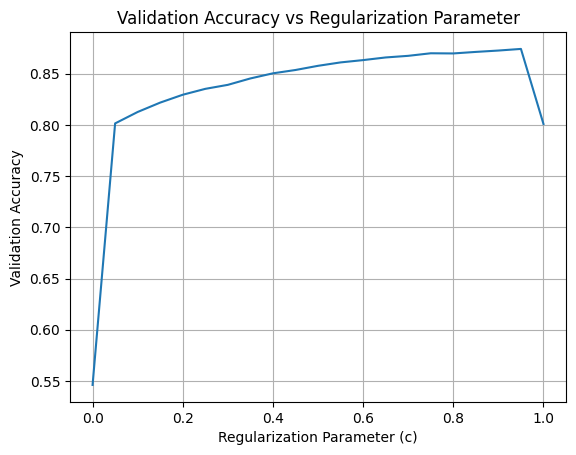
\includegraphics[width=1\textwidth]{hw3_13b.png} 
\caption{Results from c value testing}
\end{figure}

\newpage
\parbox{\textwidth}{\textbf{Solution 13 (c)}}
\noindent\rule{\textwidth}{0.4pt}\\
\begin{itemize}
    \item \parbox{\textwidth}{The model with $c=0.95$ predicted 1178 out of 10,000 incorrectly.}\\
    \item \parbox{\textwidth}{Therefore, the error rate on the MNIST test set was 0.1178 or 11.78\%.}\\
    \item \parbox{\textwidth}{Note: The accuracy of the model on the MNIST test set (88.22\%) was very close to accuracy on the training set(87.42)\%.}\\
\end{itemize}

\newpage
\parbox{\textwidth}{\textbf{Solution 13 (d)}}

\noindent\rule{\textwidth}{0.4pt}\\
\begin{figure}[H]
    \centering
    \begin{subfigure}[b]{0.3\textwidth}
        \centering
        
\includegraphics[width=\textwidth]{digit1.png}
        \caption{5 classified as 3}
        \label{fig:digit1}
    \end{subfigure}
    \hfill
    \begin{subfigure}[b]{0.3\textwidth}
        \centering
        
\includegraphics[width=\textwidth]{digit2.png}
        \caption{3 classified as 2}
        \label{fig:digit2}
    \end{subfigure}
    \hfill
    \begin{subfigure}[b]{0.3\textwidth}
        \centering
        
\includegraphics[width=\textwidth]{digit3.png}
        \caption{5 classified as 8}
        \label{fig:digit3}
    \end{subfigure}
    
    \vspace{1cm}
    
    \begin{subfigure}[b]{0.3\textwidth}
        \centering
        
\includegraphics[width=\textwidth]{digit4.png}
        \caption{1 classified as 8}
        \label{fig:digit4}
    \end{subfigure}
    \hfill
    \begin{subfigure}[b]{0.3\textwidth}
        \centering
        
\includegraphics[width=\textwidth]{digit5.png}
        \caption{5 classified as 8}
        \label{fig:digit5}
    \end{subfigure}

    \caption{Examples of misclassified digits from the test set}
    \label{fig:misclassified}
\end{figure}
\end{document}
